\section{特征向量与特征值}

\subsection{特征值与特征向量}

矩阵乘法通常会同时改变向量的长度和方向。取
\[
A=\begin{pmatrix}2&1\\1&2\end{pmatrix},\qquad
\mathbf{x}=\begin{pmatrix}1\\2\end{pmatrix},
\]
则 \(A\mathbf{x}=(4,5)^{\mathrm{T}}\)，与 \((1,2)^{\mathrm{T}}\) 不同向。但换两个向量试试：
\[
A\begin{pmatrix}1\\1\end{pmatrix}=\begin{pmatrix}3\\3\end{pmatrix}=3\begin{pmatrix}1\\1\end{pmatrix},
\qquad
A\begin{pmatrix}1\\-1\end{pmatrix}=\begin{pmatrix}1\\-1\end{pmatrix}=1\begin{pmatrix}1\\-1\end{pmatrix}.
\]
这两个方向被 \(A\) 作用后仍留在原来的直线上，只是长度变了。找这种“不被扭弯”的方向，就是本章要解决的问题。

\begin{center}
\begin{tikzpicture}
\begin{axis}[
  width=0.62\linewidth, height=5.8cm, axis equal image, axis lines=middle,
  xmin=-3.4, xmax=3.4, ymin=-3.4, ymax=3.4,
  xlabel={$x$}, ylabel={$y$}, font=\footnotesize, ticks=none,
]
\addplot[gray, thick, dashed, domain=0:360, samples=160] ({cos(x)},{sin(x)});
\addplot[blue, thick, domain=0:360, samples=240]
  ({(3*cos(x)+sin(x))/1.41421356},{(3*cos(x)-sin(x))/1.41421356});
\draw[->,red,thick] (axis cs:0,0) -- (axis cs:0.7071,0.7071)
  node[above right,font=\scriptsize]{$\mathbf{q}_1$};
\draw[->,red,thick] (axis cs:0,0) -- (axis cs:2.1213,2.1213)
  node[above right,font=\scriptsize]{$3\mathbf{q}_1$};
\draw[->,blue,thick] (axis cs:0,0) -- (axis cs:0.7071,-0.7071)
  node[below right,font=\scriptsize]{$\mathbf{q}_2$};
\node[font=\scriptsize,blue] at (axis cs:0,-2.85) {$A$ 把单位圆映成椭圆};
\end{axis}
\end{tikzpicture}
\end{center}
\centerline{\parbox{\dimexpr\linewidth-4em\relax}{\centering\footnotesize 单位圆（灰虚线）经 \(A\) 映成椭圆（蓝线）。沿 \(\mathbf{q}_1=(1,1)^{\mathrm{T}}/\sqrt2\) 方向被拉长 \(3\) 倍，沿 \(\mathbf{q}_2=(1,-1)^{\mathrm{T}}/\sqrt2\) 方向长度不变；其余方向的向量都会拐弯。}}

\begin{mydef}{特征值与特征向量}{eigenvalue-eigenvector}
设 \(A\) 为 \(n\) 阶方阵。若存在数 \(\lambda\) 和非零列向量 \(\mathbf{x}\)，使得
\[
A\mathbf{x}=\lambda\mathbf{x},
\]
则称 \(\lambda\) 为 \(A\) 的\textbf{特征值}（eigenvalue），\(\mathbf{x}\) 为属于 \(\lambda\) 的\textbf{特征向量}（eigenvector）。

把等式移项得 \((\lambda I-A)\mathbf{x}=\mathbf{0}\)。这是关于 \(\mathbf{x}\) 的齐次线性方程组，有非零解当且仅当
\[
|\lambda I-A|=0.
\]
这个方程称为 \(A\) 的\textbf{特征方程}，左端的行列式是 \(\lambda\) 的多项式。
\end{mydef}

特征向量必须非零，否则任何 \(\lambda\) 都满足 \(A\mathbf{x}=\lambda\mathbf{x}\)，定义就失去意义。特征值则可以是零：\(\lambda=0\) 时 \(A\mathbf{x}=\mathbf{0}\)，说明 \(A\) 有非零的零空间，即 \(A\) 不可逆。

同一个特征值 \(\lambda\) 的全部特征向量，再添上零向量，构成齐次方程组 \((\lambda I-A)\mathbf{x}=\mathbf{0}\) 的解空间，称为 \(\lambda\) 的\textbf{特征子空间}，记作 \(V_\lambda\)。它的维数就是属于 \(\lambda\) 的线性无关特征向量的最大个数。

\begin{formula}{求特征值与特征向量的步骤}{eigen-computation}
\begin{enumerate}
  \item 计算特征多项式 \(f(\lambda)=|\lambda I-A|\)，解 \(f(\lambda)=0\) 得到全部特征值。
  \item 对每个特征值 \(\lambda_i\)，解齐次方程组 \((\lambda_i I-A)\mathbf{x}=\mathbf{0}\)，取基础解系，得到属于 \(\lambda_i\) 的一组线性无关特征向量。全部非零线性组合都是属于 \(\lambda_i\) 的特征向量。
\end{enumerate}
\end{formula}

\textbf{例} 对上面的 \(A=\begin{pmatrix}2&1\\1&2\end{pmatrix}\)，先算
\[
|\lambda I-A|=
\begin{vmatrix}\lambda-2&-1\\-1&\lambda-2\end{vmatrix}
=(\lambda-2)^2-1=(\lambda-3)(\lambda-1),
\]
特征值为 \(3\) 和 \(1\)。

当 \(\lambda=3\) 时，
\[
(3I-A)\mathbf{x}=\begin{pmatrix}1&-1\\-1&1\end{pmatrix}
\begin{pmatrix}x_1\\x_2\end{pmatrix}=\mathbf{0},
\]
即 \(x_1=x_2\)，全部特征向量为 \(k(1,1)^{\mathrm{T}}\;(k\neq0)\)。

当 \(\lambda=1\) 时，
\[
(I-A)\mathbf{x}=\begin{pmatrix}-1&-1\\-1&-1\end{pmatrix}
\begin{pmatrix}x_1\\x_2\end{pmatrix}=\mathbf{0},
\]
即 \(x_1+x_2=0\)，全部特征向量为 \(k(1,-1)^{\mathrm{T}}\;(k\neq0)\)。

这两组解正好对应图中的两个特征方向。

有几点性质后面会反复用到。第一，若 \(\mathbf{x}\) 是特征向量，则 \(k\mathbf{x}\;(k\neq0)\) 也是同一特征值的特征向量，所以特征向量总是成整条直线出现，写答案时用通解表示。

第二，属于不同特征值的特征向量一定线性无关。设 \(\lambda_1,\dots,\lambda_m\) 互不相同，\(\mathbf{x}_i\) 属于 \(\lambda_i\)。若它们线性相关，取一个项数最少的非平凡关系
\[
c_1\mathbf{x}_1+\cdots+c_k\mathbf{x}_k=\mathbf{0}.
\]
两边左乘 \(A-\lambda_k I\)，利用 \(A\mathbf{x}_i=\lambda_i\mathbf{x}_i\)，得到
\[
c_1(\lambda_1-\lambda_k)\mathbf{x}_1+\cdots+c_{k-1}(\lambda_{k-1}-\lambda_k)\mathbf{x}_{k-1}=\mathbf{0},
\]
项数少了一项。反复这样做会把关系压到只剩一项，与该系数非零矛盾。

第三，若 \(A\mathbf{x}=\lambda\mathbf{x}\)，则
\[
A^2\mathbf{x}=\lambda^2\mathbf{x},\qquad A^k\mathbf{x}=\lambda^k\mathbf{x},
\]
对任意多项式 \(g(t)\) 也有 \(g(A)\mathbf{x}=g(\lambda)\mathbf{x}\)。也就是说，\(g(\lambda)\) 是 \(g(A)\) 的特征值，且 \(\mathbf{x}\) 仍是对应的特征向量。这条性质是后面计算矩阵幂和矩阵多项式的依据。

把这些性质串起来，还能得到两个常用结论。若 \(A\) 可逆，则 \(\lambda\neq0\)，在 \(A\mathbf{x}=\lambda\mathbf{x}\) 两边左乘 \(A^{-1}\)，得
\[
A^{-1}\mathbf{x}=\frac1\lambda\mathbf{x},
\]
所以 \(A^{-1}\) 的特征值是 \(1/\lambda\)，特征向量仍是 \(\mathbf{x}\)。伴随矩阵满足 \(A^*=|A|A^{-1}\)（\(A\) 可逆时），因此 \(A^*\) 的特征值是 \(|A|/\lambda\)，特征向量同样不变。

\subsection{特征多项式}

特征多项式定义为
\[
f(\lambda)=|\lambda I-A|=
\begin{vmatrix}
\lambda-a_{11}&-a_{12}&\cdots&-a_{1n}\\
-a_{21}&\lambda-a_{22}&\cdots&-a_{2n}\\
\vdots&\vdots&\ddots&\vdots\\
-a_{n1}&-a_{n2}&\cdots&\lambda-a_{nn}
\end{vmatrix}.
\]
它是首项系数为 \(1\) 的 \(n\) 次多项式。完整展开很麻烦，但有两个系数可以直接读出来：
\[
f(\lambda)=\lambda^n-(\operatorname{tr}A)\lambda^{n-1}+\cdots+(-1)^n|A|.
\]
其中 \(\operatorname{tr}A=a_{11}+a_{22}+\cdots+a_{nn}\) 是主对角线元素之和，称为 \(A\) 的\textbf{迹}。

理由不难看出：在对角线乘积 \(\prod_i(\lambda-a_{ii})\) 中，\(\lambda^{n-1}\) 项来自 \(n-1\) 个因子取 \(\lambda\)、剩下一个因子取 \(-a_{ii}\)，系数正好是 \(-\sum_i a_{ii}\)；其他展开项的 \(\lambda\) 次数最多为 \(n-2\)。常数项则令 \(\lambda=0\) 直接得到 \(|{-A}|=(-1)^n|A|\)。

设 \(A\) 的 \(n\) 个特征值（重根按重数计）为 \(\lambda_1,\dots,\lambda_n\)。由韦达定理，
\[
\lambda_1+\cdots+\lambda_n=\operatorname{tr}A,\qquad
\lambda_1\lambda_2\cdots\lambda_n=|A|.
\]
这两个等式是最快的验算工具：特征值算完，先看和是否等于迹、积是否等于行列式，能拦住大部分算术错误。

\begin{center}
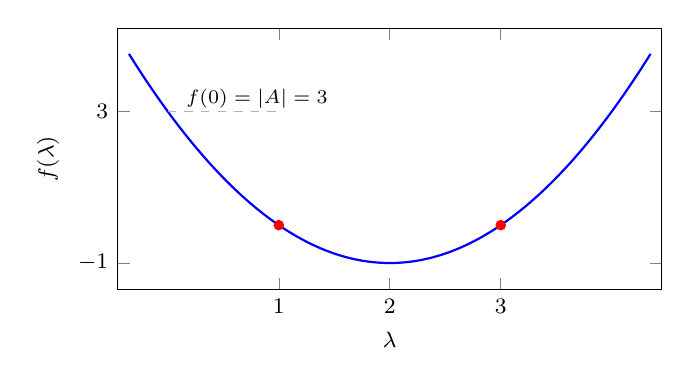
\begin{tikzpicture}
\begin{axis}[
  width=0.7\linewidth, height=4.9cm,
  xmin=-0.45, xmax=4.45, ymin=-1.7, ymax=5.2,
  xlabel={$\lambda$}, ylabel={$f(\lambda)$},
  xtick={1,2,3}, ytick={-1,3},
  font=\footnotesize, clip=false,
]
\addplot[blue, thick, domain=-0.35:4.35, samples=140]{x^2-4*x+3};
\addplot[only marks, mark=*, mark size=1.7pt, red] coordinates {(1,0)(3,0)};
\draw[dashed,gray!60] (axis cs:0,3) -- (axis cs:1,3);
\node[font=\scriptsize,anchor=west] at (axis cs:0.08,3.35) {$f(0)=|A|=3$};
\end{axis}
\end{tikzpicture}
\end{center}
\centerline{\parbox{\dimexpr\linewidth-4em\relax}{\centering\footnotesize \(f(\lambda)=\lambda^2-4\lambda+3\) 的图像。曲线与横轴的交点就是特征值 \(1\) 和 \(3\)，与纵轴的交点 \(f(0)=3\) 等于 \(|A|\)。两根之和 \(4\) 正是迹；根的位置和这两个系数互相牵制。}}

Cayley--Hamilton 定理把这个多项式与矩阵本身联系起来：把 \(\lambda\) 换成 \(A\)，结果竟然是零矩阵。

\begin{conclusion}{Cayley--Hamilton 定理}{cayley-hamilton}
设 \(A\) 是 \(n\) 阶方阵，\(f(\lambda)=|\lambda I-A|\) 是它的特征多项式，则
\[
f(A)=O.
\]
即任意方阵都满足自己的特征方程。
\end{conclusion}

对上面的二阶例子，\(f(\lambda)=\lambda^2-4\lambda+3\)，于是 \(A^2-4A+3I=O\)。这条式子有两个直接用途。

一是降次：把 \(A^2\) 写成 \(4A-3I\)，再乘 \(A\) 就能把 \(A^3\) 也表示成 \(A\) 与 \(I\) 的组合，如此递推，任意高次幂都能降到一次。

二是求逆。因为 \(A^2-4A+3I=O\)，移项得
\[
A(4I-A)=3I,\qquad\text{所以}\qquad
A^{-1}=\frac13(4I-A)=\frac13\begin{pmatrix}2&-1\\-1&2\end{pmatrix}.
\]
这与用伴随矩阵算出的结果一致。注意前提是常数项 \((-1)^n|A|\neq0\)，否则 \(A\) 本来就不可逆。

\subsection{相似与对角化}

同一个线性变换，换一组基，矩阵就换一副样子。设 \(P\) 的列是新基，向量在新基下的坐标是 \(\mathbf{y}=P^{-1}\mathbf{x}\)，那么
\[
A\mathbf{x}=AP\mathbf{y}=P(P^{-1}AP)\mathbf{y}.
\]
所以线性变换在新基下的矩阵是 \(P^{-1}AP\)。

\begin{mydef}{相似矩阵}{similar-matrices}
设 \(A,B\) 为 \(n\) 阶方阵。若存在可逆矩阵 \(P\)，使得
\[
B=P^{-1}AP,
\]
则称 \(A\) 与 \(B\) \textbf{相似}，记作 \(A\sim B\)。变换 \(A\mapsto P^{-1}AP\) 称为相似变换。
\end{mydef}

相似矩阵有相同的特征多项式：
\[
|\lambda I-P^{-1}AP|
=|P^{-1}(\lambda I-A)P|
=|P^{-1}|\,|\lambda I-A|\,|P|
=|\lambda I-A|.
\]
因此它们的特征值（包括代数重数）、迹、行列式都相同；秩也相同，因为左右乘可逆矩阵不改变秩。

转置也有相同的特征多项式：
\[
|\lambda I-A^{\mathrm{T}}|=|(\lambda I-A)^{\mathrm{T}}|=|\lambda I-A|,
\]
所以 \(A\) 与 \(A^{\mathrm{T}}\) 的特征值相同，但特征向量一般不同。这一点常被用来计算与转置有关的题目。

反过来不成立。单位矩阵 \(I\) 与 \(J=\begin{pmatrix}1&1\\0&1\end{pmatrix}\) 的特征值都是 \(1,1\)，但 \(I\) 只与自己相似，\(J\neq I\)，所以二者不相似。特征值相同只是相似的必要条件；要判断相似，还得看特征向量的结构。

对角化是相似变换里最省事的一种：把矩阵化成对角形。

\begin{mydef}{可对角化}{diagonalizable}
若 \(n\) 阶方阵 \(A\) 相似于对角矩阵，即存在可逆矩阵 \(P\) 和数 \(\lambda_1,\dots,\lambda_n\)，使得
\[
P^{-1}AP=\operatorname{diag}(\lambda_1,\dots,\lambda_n),
\]
则称 \(A\) \textbf{可对角化}。
\end{mydef}

设 \(P=(\mathbf{p}_1,\dots,\mathbf{p}_n)\)，\(\Lambda=\operatorname{diag}(\lambda_1,\dots,\lambda_n)\)。等式 \(P^{-1}AP=\Lambda\) 等价于 \(AP=P\Lambda\)。逐列看，就是
\[
A\mathbf{p}_j=\lambda_j\mathbf{p}_j,\qquad j=1,\dots,n.
\]
所以 \(P\) 的每一列都必须是 \(A\) 的特征向量，而且 \(P\) 可逆要求这 \(n\) 列线性无关。反过来，只要能凑出 \(n\) 个线性无关的特征向量，按顺序排成 \(P\)，对角元按同样顺序排成 \(\Lambda\)，就完成了对角化。

问题归结为：特征向量够不够用？这要用重数来回答。特征值 \(\lambda_0\) 作为特征多项式根的重数，称为它的\textbf{代数重数} \(m_a(\lambda_0)\)；特征子空间 \(V_{\lambda_0}\) 的维数，称为它的\textbf{几何重数} \(m_g(\lambda_0)\)。两者总有
\[
1\le m_g(\lambda_0)\le m_a(\lambda_0).
\]
几何重数不超过代数重数，这个不等式要用 Jordan 标准形或广义特征子空间来证明，这里先记住结论。

\begin{conclusion}{可对角化的充要条件}{diagonalizable-criterion}
\(n\) 阶方阵 \(A\) 可对角化，当且仅当
\[
\sum_{\lambda_0} m_g(\lambda_0)=n,
\]
等价地说，每个特征值都满足 \(m_g(\lambda_0)=m_a(\lambda_0)\)。

特别地，若 \(A\) 有 \(n\) 个互不相同的特征值，则 \(A\) 一定可对角化；这只是充分条件，不是必要条件。
\end{conclusion}

看一个不可对角化的例子：
\[
A=\begin{pmatrix}1&2\\0&1\end{pmatrix}.
\]
特征多项式是 \((\lambda-1)^2\)，所以 \(\lambda=1\) 的代数重数为 \(2\)。但
\[
A-I=\begin{pmatrix}0&2\\0&0\end{pmatrix}
\]
的秩为 \(1\)，零空间维数为 \(2-1=1\)，即几何重数只有 \(1\)。属于 \(1\) 的特征向量只有 \(k(1,0)^{\mathrm{T}}\) 这一条直线，凑不出两组线性无关的特征向量，因此 \(A\) 不可对角化。

\begin{center}
\begin{tikzpicture}
\begin{axis}[
  width=0.62\linewidth, height=5.2cm, axis equal image, axis lines=middle,
  xmin=-0.35, xmax=3.45, ymin=-0.45, ymax=1.75,
  xlabel={$x$}, ylabel={$y$}, font=\footnotesize, ticks=none,
]
\draw[gray!40, fill=gray!12, thick] (axis cs:0,0) rectangle (axis cs:1,1);
\draw[blue, thick] (axis cs:0,0) -- (axis cs:1,0) -- (axis cs:3,1) -- (axis cs:2,1) -- cycle;
\draw[->,red,thick] (axis cs:0,0) -- (axis cs:1,0)
  node[below,font=\scriptsize]{$\mathbf{p}_1$};
\draw[->,orange!80!black,thick] (axis cs:0,1) -- (axis cs:2,1)
  node[anchor=south,font=\scriptsize]{$A\mathbf{e}_2$};
\node[font=\scriptsize,blue] at (axis cs:2.35,1.5) {$A=\begin{pmatrix}1&2\\0&1\end{pmatrix}$};
\end{axis}
\end{tikzpicture}
\end{center}
\centerline{\parbox{\dimexpr\linewidth-4em\relax}{\centering\footnotesize 剪切矩阵把单位正方形（灰）压成平行四边形（蓝）。水平方向的向量不动，这是唯一的特征方向；竖直向量被推斜。一个方向撑不起整个平面，所以找不到两组线性无关的特征向量，矩阵不能对角化。}}

若 \(A\) 可对角化，\(P^{-1}AP=\Lambda\) 的几何含义是：在由特征向量组成的基下，\(A\) 只沿各个基方向独立伸缩，不再混合坐标。这也是后面算 \(A^k\)、解微分方程组时总想先对角化的原因。
\subsection{实对称矩阵的谱分解}

实对称矩阵是满足 \(A=A^{\mathrm{T}}\) 的实方阵。这类矩阵的对角化不需要额外条件，而且得到的特征向量还能选成标准正交基。

先看三个基本事实。

\textbf{特征值全是实数。} 设 \(A\mathbf{x}=\lambda\mathbf{x}\)，其中 \(\mathbf{x}\) 是非零复向量。两边左乘 \(\overline{\mathbf{x}}^{\mathrm{T}}\)，得
\[
\overline{\mathbf{x}}^{\mathrm{T}}A\mathbf{x}
=\lambda\,\overline{\mathbf{x}}^{\mathrm{T}}\mathbf{x}.
\]
左端是一个数，且
\[
\overline{\overline{\mathbf{x}}^{\mathrm{T}}A\mathbf{x}}
=\mathbf{x}^{\mathrm{T}}A\overline{\mathbf{x}}
=(A\mathbf{x})^{\mathrm{T}}\overline{\mathbf{x}}
=\overline{\mathbf{x}}^{\mathrm{T}}A\mathbf{x},
\]
所以左端为实数；而 \(\overline{\mathbf{x}}^{\mathrm{T}}\mathbf{x}>0\)，故 \(\lambda\) 为实数。

\textbf{不同特征值的特征向量正交。} 设 \(A\mathbf{x}=\lambda_1\mathbf{x}\)，\(A\mathbf{y}=\lambda_2\mathbf{y}\)，且 \(\lambda_1\neq\lambda_2\)。则
\[
\lambda_1\mathbf{x}\cdot\mathbf{y}
=(A\mathbf{x})\cdot\mathbf{y}
=\mathbf{x}\cdot(A\mathbf{y})
=\lambda_2\mathbf{x}\cdot\mathbf{y}.
\]
移项得 \((\lambda_1-\lambda_2)\mathbf{x}\cdot\mathbf{y}=0\)，故 \(\mathbf{x}\cdot\mathbf{y}=0\)。

\textbf{一定存在标准正交的特征向量基。} 这是谱定理的内容。

\begin{conclusion}{实对称矩阵的谱定理}{spectral-theorem}
设 \(A\) 是 \(n\) 阶实对称矩阵，则存在正交矩阵 \(Q\)（即 \(Q^{\mathrm{T}}Q=I\)），使得
\[
Q^{\mathrm{T}}AQ=Q^{-1}AQ=\operatorname{diag}(\lambda_1,\dots,\lambda_n),
\]
其中 \(\lambda_1,\dots,\lambda_n\) 是 \(A\) 的全部特征值，均为实数。\(Q\) 的列是两两正交的单位特征向量，构成 \(\mathbb{R}^n\) 的一组标准正交基。
\end{conclusion}

由谱定理，实对称矩阵一定可对角化，且 \(\operatorname{r}(A)\) 等于非零特征值的个数（重数计入）。

求 \(Q\) 的步骤与一般对角化相同，只是多了正交化和单位化：
\begin{formula}{实对称矩阵的正交对角化步骤}{orthogonal-diagonalization}
\begin{enumerate}
  \item 解 \(|\lambda I-A|=0\)，求出全部特征值。
  \item 对每个特征值解 \((\lambda I-A)\mathbf{x}=\mathbf{0}\)，取基础解系。
  \item 若某个特征值重数大于 \(1\)，对它对应的基础解系做 Gram--Schmidt 正交化；不同特征值的向量已经自动正交，不必再处理。
  \item 把所有特征向量单位化，按列排成 \(Q\)，则 \(Q^{\mathrm{T}}AQ=\operatorname{diag}(\lambda_1,\dots,\lambda_n)\)，对角元的顺序与 \(Q\) 的列一一对应。
\end{enumerate}
\end{formula}

对前面的 \(A=\begin{pmatrix}2&1\\1&2\end{pmatrix}\)，属于 \(3\) 的单位特征向量是
\[
\mathbf{q}_1=\frac1{\sqrt2}\begin{pmatrix}1\\1\end{pmatrix},
\]
属于 \(1\) 的单位特征向量是
\[
\mathbf{q}_2=\frac1{\sqrt2}\begin{pmatrix}1\\-1\end{pmatrix}.
\]
它们正交。取
\[
Q=(\mathbf{q}_1,\mathbf{q}_2)=\frac1{\sqrt2}\begin{pmatrix}1&1\\1&-1\end{pmatrix},
\]
则
\[
Q^{\mathrm{T}}AQ=\begin{pmatrix}3&0\\0&1\end{pmatrix}.
\]

把 \(Q^{\mathrm{T}}AQ=\Lambda\) 两边左乘 \(Q\)、右乘 \(Q^{\mathrm{T}}\)，得到
\[
A=Q\Lambda Q^{\mathrm{T}}
=\lambda_1\mathbf{q}_1\mathbf{q}_1^{\mathrm{T}}
+\lambda_2\mathbf{q}_2\mathbf{q}_2^{\mathrm{T}}
+\cdots+
\lambda_n\mathbf{q}_n\mathbf{q}_n^{\mathrm{T}}.
\]
这就是\textbf{谱分解}。每一项 \(\mathbf{q}_i\mathbf{q}_i^{\mathrm{T}}\) 是一个秩一矩阵。记 \(P_i=\mathbf{q}_i\mathbf{q}_i^{\mathrm{T}}\)，它把向量投影到 \(\mathbf{q}_i\) 方向上；不同项的投影矩阵互相正交，即 \(P_iP_j=O\;(i\neq j)\)。所以谱分解把 \(A\) 拆成了若干个互不干扰的一维伸缩。

对上面的二阶例子，直接验证：
\[
A=3\cdot\frac12\begin{pmatrix}1&1\\1&1\end{pmatrix}
+1\cdot\frac12\begin{pmatrix}1&-1\\-1&1\end{pmatrix}
=\begin{pmatrix}2&1\\1&2\end{pmatrix}.
\]

\begin{center}
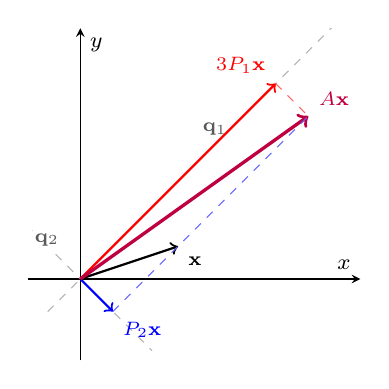
\begin{tikzpicture}
\begin{axis}[
  width=0.66\linewidth, height=5.8cm, axis equal image, axis lines=middle,
  xmin=-0.8, xmax=4.3, ymin=-1.25, ymax=3.85,
  xlabel={$x$}, ylabel={$y$}, font=\footnotesize, ticks=none,
]
\draw[dashed,gray!60] (axis cs:-0.5,-0.5) -- (axis cs:3.9,3.9);
\draw[dashed,gray!60] (axis cs:-1.1,1.1) -- (axis cs:1.1,-1.1);
\node[gray!70!black,font=\scriptsize,fill=white,inner sep=1pt,anchor=south east] at (axis cs:2.3,2.15) {$\mathbf{q}_1$};
\node[gray!70!black,font=\scriptsize,fill=white,inner sep=1pt,anchor=north west] at (axis cs:-0.75,0.75) {$\mathbf{q}_2$};
\draw[->,red,thick] (axis cs:0,0) -- (axis cs:3,3)
  node[anchor=south east,font=\scriptsize]{$3P_1\mathbf{x}$};
\draw[->,blue,thick] (axis cs:0,0) -- (axis cs:0.5,-0.5)
  node[anchor=north west,font=\scriptsize]{$P_2\mathbf{x}$};
\draw[->,black,thick] (axis cs:0,0) -- (axis cs:1.5,0.5)
  node[anchor=north west,font=\scriptsize]{$\mathbf{x}$};
\draw[->,purple,very thick] (axis cs:0,0) -- (axis cs:3.5,2.5)
  node[anchor=south west,font=\scriptsize]{$A\mathbf{x}$};
\draw[dashed,red!60] (axis cs:3,3) -- (axis cs:3.5,2.5);
\draw[dashed,blue!60] (axis cs:0.5,-0.5) -- (axis cs:3.5,2.5);
\end{axis}
\end{tikzpicture}
\end{center}
\centerline{\parbox{\dimexpr\linewidth-4em\relax}{\centering\footnotesize 取 \(\mathbf{x}=(1.5,0.5)^{\mathrm{T}}\)。先投影到 \(\mathbf{q}_1,\mathbf{q}_2\) 两个正交方向，得到 \(P_1\mathbf{x}=(1,1)^{\mathrm{T}}\) 和 \(P_2\mathbf{x}=(0.5,-0.5)^{\mathrm{T}}\)；分别乘 \(\lambda_1=3\)、\(\lambda_2=1\) 后相加，正好得到 \(A\mathbf{x}=(3.5,2.5)^{\mathrm{T}}\)。虚线平行四边形就是这个加法。}}

谱分解在实际问题里很常见。若 \(A\) 是数据的协方差矩阵，\(\lambda_i\) 表示数据沿主轴 \(\mathbf{q}_i\) 方向的方差，\(\lambda_i/\sum_j\lambda_j\) 就是该主成分解释的方差比例，这正是主成分分析的出发点。在二次型 \(f(\mathbf{x})=\mathbf{x}^{\mathrm{T}}A\mathbf{x}\) 中，令 \(\mathbf{x}=Q\mathbf{y}\) 后交叉项全部消失，只剩 \(\sum_i\lambda_i y_i^2\)，曲面的主轴方向和伸缩比例也由特征值给出。

\subsection{矩阵幂的计算}

对角化最直接的用途是算高次幂。若 \(A=P\Lambda P^{-1}\)，则
\[
A^k=P\Lambda^kP^{-1}
=P\operatorname{diag}(\lambda_1^k,\dots,\lambda_n^k)P^{-1}.
\]
中间展开时 \(P^{-1}P\) 两两抵消，只剩 \(k\) 个 \(\Lambda\) 相乘。对角矩阵的乘法就是对角元各自相乘，所以求 \(A^k\) 变成求 \(n\) 个数的 \(k\) 次方。

对 \(A=\begin{pmatrix}2&1\\1&2\end{pmatrix}\)，用前面得到的 \(Q\) 和 \(\Lambda=\operatorname{diag}(3,1)\)：
\[
A^k=Q\begin{pmatrix}3^k&0\\0&1\end{pmatrix}Q^{\mathrm{T}}
=\frac12
\begin{pmatrix}
3^k+1&3^k-1\\
3^k-1&3^k+1
\end{pmatrix}.
\]
令 \(k=1\)，右边是 \(\frac12\begin{pmatrix}4&2\\2&4\end{pmatrix}=\begin{pmatrix}2&1\\1&2\end{pmatrix}\)，与 \(A\) 一致；令 \(k=0\)，右边是 \(I\)。这两个特殊值可以快速检查公式有没有写错。

当 \(k\) 很大时，\(3^k\) 远大于 \(1^k\)，于是
\[
A^k\approx\frac{3^k}{2}\begin{pmatrix}1&1\\1&1\end{pmatrix}
=3^k\mathbf{q}_1\mathbf{q}_1^{\mathrm{T}}.
\]
主导项就是最大特征值对应的那个投影。这也解释了为什么迭代 \(A^k\mathbf{x}\) 的方向会越来越靠近主特征向量：其他方向按 \((\lambda_i/\lambda_1)^k\) 衰减掉了。

\begin{center}
\begin{tikzpicture}
\begin{axis}[
  width=0.72\linewidth, height=4.9cm,
  xmin=-0.25, xmax=6.35, ymin=0, ymax=48,
  xlabel={$k$}, ylabel={方向角（度）},
  xtick={0,1,2,3,4,5,6}, ytick={0,15,30,45},
  font=\footnotesize, clip=false,
]
\addplot[blue, thick, mark=*, mark size=1.5pt] coordinates {
  (0,0) (1,26.565) (2,38.660) (3,42.878)
  (4,44.292) (5,44.763) (6,44.922)
};
\draw[dashed,gray!70] (axis cs:0,45) -- (axis cs:6.35,45);
\node[font=\scriptsize,anchor=south east] at (axis cs:6.3,45.4) {$45^\circ$ 渐近线};
\end{axis}
\end{tikzpicture}
\end{center}
\centerline{\parbox{\dimexpr\linewidth-4em\relax}{\centering\footnotesize \(A^k\mathbf{e}_1\) 与 \(x\) 轴的夹角随 \(k\) 的变化。角度单调上升并逼近 \(45^\circ\)，也就是 \(\mathbf{q}_1\) 的方向；误差每步按 \(|\lambda_2/\lambda_1|=1/3\) 缩小，所以曲线先快后慢。特征值比值越小，曲线越早贴近渐近线。}}

若 \(A\) 不可对角化，也有办法。先看只有一个特征值 \(\lambda\) 的情形（多个特征值可以按 Jordan 块分开处理），此时可写成
\[
A=\lambda I+N,
\]
其中 \(N=A-\lambda I\) 是幂零矩阵，即某个 \(N^m=O\)。由于 \(\lambda I\) 与任何矩阵都交换，二项式定理仍然成立：
\[
A^k=(\lambda I+N)^k
=\sum_{j=0}^{k}\binom{k}{j}\lambda^{k-j}N^j.
\]
当 \(j\ge m\) 时 \(N^j=O\)，所以求和其实只有前 \(m\) 项；当 \(\lambda\neq0\) 时，它是一个关于 \(k\) 的多项式乘以 \(\lambda^k\)。

例如
\[
A=\begin{pmatrix}2&1\\0&2\end{pmatrix}=2I+N,\qquad
N=\begin{pmatrix}0&1\\0&0\end{pmatrix},\quad N^2=O.
\]
于是
\[
A^k=2^kI+k\,2^{k-1}N
=\begin{pmatrix}2^k&k\,2^{k-1}\\0&2^k\end{pmatrix}.
\]
对角线上仍是 \(2^k\)，但右上角多出一个随 \(k\) 线性增长的项，这正是不可对角化带来的差别。

秩一矩阵还有更快的公式。若 \(A=\mathbf{u}\mathbf{v}^{\mathrm{T}}\)，则
\[
A^2=\mathbf{u}\mathbf{v}^{\mathrm{T}}\mathbf{u}\mathbf{v}^{\mathrm{T}}
=(\mathbf{v}^{\mathrm{T}}\mathbf{u})\,\mathbf{u}\mathbf{v}^{\mathrm{T}}
=(\mathbf{v}^{\mathrm{T}}\mathbf{u})A,
\]
所以
\[
A^k=(\mathbf{v}^{\mathrm{T}}\mathbf{u})^{k-1}A\qquad(k\ge1).
\]
一个数 \(\mathbf{v}^{\mathrm{T}}\mathbf{u}\) 就决定了整个幂序列。

Cayley--Hamilton 定理则提供了另一条降次途径：把 \(A^n\) 用 \(I,A,\dots,A^{n-1}\) 表示，再递推高次幂。矩阵阶数不高、幂次也不高时，这比求特征向量更省事。

最后提一句更一般的图景。在复数域上，任何方阵都相似于一个 Jordan 标准形：对角线上是特征值，对角线上方可能有 \(1\)。Jordan 块的个数等于几何重数，最大块的阶数刻画了“不能对角化”的程度。再往外，Gershgorin 圆盘定理用对角元和行内非对角元绝对值之和，在复平面上圈出特征值所在的区域。这两部分超出考研主线，知道结论即可。

\newpage
\section{习题}

\subsection{本章速览}

\begin{itemize}
  \item \textbf{定义}：若 \(A\mathbf{x}=\lambda\mathbf{x}\) 且 \(\mathbf{x}\neq\mathbf{0}\)，则称 \(\lambda\) 为 \(A\) 的特征值，\(\mathbf{x}\) 为属于 \(\lambda\) 的特征向量。特征值由 \(|\lambda I-A|=0\) 求出，特征向量是 \((\lambda I-A)\mathbf{x}=\mathbf{0}\) 的全部非零解；特征向量必须非零，而特征值可以为零。
  \item \textbf{特征多项式}：\(f(\lambda)=|\lambda I-A|=\lambda^n-(\operatorname{tr}A)\lambda^{n-1}+\cdots+(-1)^n|A|\)。因此 \(\sum\lambda_i=\operatorname{tr}A\)，\(\prod\lambda_i=|A|\)，这两条是检验特征值算得对不对的最快方法。
  \item \textbf{相似}：\(B=P^{-1}AP\)（\(P\) 可逆）。相似矩阵有相同的特征多项式、特征值（含重数）、迹、行列式和秩；但特征值相同只是相似的必要条件，不能反推相似。
  \item \textbf{可对角化}：\(A\) 相似于对角矩阵，当且仅当 \(A\) 有 \(n\) 个线性无关的特征向量，等价于每个特征值都满足“几何重数 \(=\) 代数重数”。\(A\) 有 \(n\) 个互不相同的特征值只是充分条件，不是必要条件。
  \item \textbf{实对称矩阵}：特征值全为实数；不同特征值对应的特征向量自动正交；一定存在正交矩阵 \(Q\)，使 \(Q^{\mathrm{T}}AQ=Q^{-1}AQ=\Lambda\)。求 \(Q\) 时只需对同一特征值内部的向量作 Schmidt 正交化，再全部单位化。
  \item \textbf{矩阵幂}：若 \(A=P\Lambda P^{-1}\)，则 \(A^n=P\Lambda^nP^{-1}\)，对角元直接取 \(n\) 次方。若 \(A\) 不可对角化，常把它拆成 \(A=\lambda I+N\)（\(N\) 幂零），用二项式定理展开；秩为 \(1\) 的矩阵 \(A=\mathbf{u}\mathbf{v}^{\mathrm{T}}\) 满足 \(A^2=(\mathbf{v}^{\mathrm{T}}\mathbf{u})A\)，可由此递推高次幂。
\end{itemize}

\subsection{基础过关题}

\textbf{1.} 判断下列说法是否正确，并说明理由：
\begin{enumerate}[label=(\arabic*)]
  \item 零矩阵 \(O\) 的特征值全为 \(0\)，且任意非零向量都是它的特征向量；
  \item 若 \(A\) 与 \(A^{\mathrm{T}}\) 有相同的特征值，则它们也有相同的特征向量；
  \item 若 \(3\) 阶矩阵 \(A\) 的特征值全为 \(0\)，则 \(A=O\)；
  \item 实对称矩阵属于不同特征值的特征向量必正交；
  \item \(n\) 阶矩阵 \(A\) 可对角化，当且仅当 \(A\) 的每个特征值的几何重数都等于其代数重数。
\end{enumerate}

\ifshowsolutions%
\boxed{\textbf{解}}
\textbf{思路：} 前四问都回到定义 \(A\mathbf{x}=\lambda\mathbf{x}\;(\mathbf{x}\neq\mathbf{0})\)，用具体反例否定错误命题；第五问复述可对角化的充要条件，并说清“方向”为什么成立。

\begin{enumerate}[label=(\arabic*)]
  \item \textbf{正确。} 对任意 \(\mathbf{x}\neq\mathbf{0}\)，有 \(O\mathbf{x}=\mathbf{0}=0\cdot\mathbf{x}\)，故 \(0\) 是特征值，且每个非零向量都是属于 \(0\) 的特征向量。
  \item \textbf{错误。} 取
  \[
  A=\begin{pmatrix}1&1\\0&2\end{pmatrix},\qquad
  A^{\mathrm{T}}=\begin{pmatrix}1&0\\1&2\end{pmatrix}.
  \]
  两者的特征值都是 \(1,2\)。但 \(A\) 的属于 \(1\) 的特征向量可取 \((1,0)^{\mathrm{T}}\)，属于 \(2\) 的可取 \((1,1)^{\mathrm{T}}\)；而 \(A^{\mathrm{T}}\) 的属于 \(1\) 的特征向量可取 \((1,-1)^{\mathrm{T}}\)，属于 \(2\) 的可取 \((0,1)^{\mathrm{T}}\)。两组特征向量没有公共的非零向量，故“特征向量相同”不成立。
  \item \textbf{错误。} 取
  \[
  N=\begin{pmatrix}0&1&0\\0&0&1\\0&0&0\end{pmatrix},\qquad N^3=O.
  \]
  \(N\) 是上三角矩阵，对角线全为 \(0\)，故特征多项式为 \(\lambda^3\)，三个特征值全为 \(0\)；但 \(N\neq O\)。这说明“特征值全为零”只能推出 \(A\) 幂零，不能推出 \(A=O\)。
  \item \textbf{正确。} 设 \(A\) 实对称，\(A\mathbf{x}=\lambda\mathbf{x}\)，\(A\mathbf{y}=\mu\mathbf{y}\)，\(\lambda\neq\mu\)，且 \(\mathbf{x},\mathbf{y}\neq\mathbf{0}\)。利用 \(A^{\mathrm{T}}=A\)，
  \[
  \lambda\,\mathbf{x}^{\mathrm{T}}\mathbf{y}
  =(A\mathbf{x})^{\mathrm{T}}\mathbf{y}
  =\mathbf{x}^{\mathrm{T}}A^{\mathrm{T}}\mathbf{y}
  =\mathbf{x}^{\mathrm{T}}A\mathbf{y}
  =\mu\,\mathbf{x}^{\mathrm{T}}\mathbf{y}.
  \]
  移项得 \((\lambda-\mu)\mathbf{x}^{\mathrm{T}}\mathbf{y}=0\)。由于 \(\lambda\neq\mu\)，只能有 \(\mathbf{x}^{\mathrm{T}}\mathbf{y}=0\)，即两向量正交。
  \item \textbf{正确。} 若 \(A\) 可对角化，即 \(P^{-1}AP=\operatorname{diag}(\lambda_1,\ldots,\lambda_n)\)，则 \(P\) 的 \(n\) 个列向量是 \(A\) 的 \(n\) 个线性无关的特征向量。对某个特征值 \(\lambda_0\)，对角矩阵中 \(\lambda_0\) 出现的次数就是它的代数重数，而 \(P\) 中属于 \(\lambda_0\) 的列正好给出个数等于代数重数的线性无关特征向量，故几何重数等于代数重数。\\
  反之，若每个特征值的几何重数都等于代数重数，把各特征值对应的特征子空间的基础解系全部合在一起，向量个数为各代数重数之和 \(n\)，且不同特征子空间的向量线性无关，于是得到 \(n\) 个线性无关的特征向量，\(A\) 可对角化。
\end{enumerate}

\boxed{\parbox{0.9\linewidth}{\raggedright\textbf{答案：}(1) 正确；(2) 错误；(3) 错误；(4) 正确；(5) 正确。}}
\else \answerarea[8] \fi%

\textbf{2.} 设
\[
A=\begin{pmatrix}0&1&1\\1&0&1\\1&1&0\end{pmatrix}.
\]
求 \(A\) 的全部特征值与特征向量，并判断 \(A\) 是否可对角化；若可对角化，求出可逆矩阵 \(P\) 和对角矩阵 \(\Lambda\)，使 \(P^{-1}AP=\Lambda\)。

\ifshowsolutions%
\boxed{\textbf{解}}
\textbf{思路：} 先算特征多项式定特征值，再逐个解 \((\lambda I-A)\mathbf{x}=\mathbf{0}\)。特征向量个数达到 \(3\) 就说明可对角化，按列拼成 \(P\) 即可。

\textbf{第一步：求特征值。}
\[
|\lambda I-A|=
\begin{vmatrix}
\lambda&-1&-1\\
-1&\lambda&-1\\
-1&-1&\lambda
\end{vmatrix}.
\]
把第 \(2,3\) 行加到第 \(1\) 行，第 \(1\) 行变为 \((\lambda-2,\lambda-2,\lambda-2)\)，提出公因子：
\[
|\lambda I-A|=(\lambda-2)
\begin{vmatrix}
1&1&1\\
-1&\lambda&-1\\
-1&-1&\lambda
\end{vmatrix}.
\]
再把第 \(2,3\) 列分别减去第 \(1\) 列：
\[
|\lambda I-A|=(\lambda-2)
\begin{vmatrix}
1&0&0\\
-1&\lambda+1&0\\
-1&0&\lambda+1
\end{vmatrix}
=(\lambda-2)(\lambda+1)^2.
\]
故特征值为 \(\lambda_1=2\)（单根），\(\lambda_2=\lambda_3=-1\)（二重根）。检验：\(\operatorname{tr}A=0=2-1-1\)，\(|A|=2\cdot(-1)\cdot(-1)=2\)。

\textbf{第二步：求特征向量。}

对 \(\lambda=2\)，解 \((2I-A)\mathbf{x}=\mathbf{0}\)：
\[
\begin{pmatrix}
2&-1&-1\\
-1&2&-1\\
-1&-1&2
\end{pmatrix}
\begin{pmatrix}x_1\\x_2\\x_3\end{pmatrix}=\mathbf{0}
\;\Longrightarrow\;
x_1=x_2=x_3.
\]
取 \(\mathbf{p}_1=(1,1,1)^{\mathrm{T}}\)，全部特征向量为 \(k_1\mathbf{p}_1\;(k_1\neq0)\)。

对 \(\lambda=-1\)，解 \((-I-A)\mathbf{x}=\mathbf{0}\)：
\[
\begin{pmatrix}-1&-1&-1\\-1&-1&-1\\-1&-1&-1\end{pmatrix}
\begin{pmatrix}x_1\\x_2\\x_3\end{pmatrix}=\mathbf{0}
\;\Longrightarrow\;
x_1+x_2+x_3=0.
\]
取基础解系 \(\mathbf{p}_2=(1,-1,0)^{\mathrm{T}}\)，\(\mathbf{p}_3=(1,0,-1)^{\mathrm{T}}\)，全部特征向量为 \(k_2\mathbf{p}_2+k_3\mathbf{p}_3\)（\(k_2,k_3\) 不全为零）。

\textbf{第三步：判断可对角化并构造 \(P\)。}
共有 \(3\) 个线性无关的特征向量（不同特征值的特征向量线性无关，同一特征值取的是基础解系），故 \(A\) 可对角化。令
\[
P=(\mathbf{p}_1,\mathbf{p}_2,\mathbf{p}_3)=
\begin{pmatrix}
1&1&1\\
1&-1&0\\
1&0&-1
\end{pmatrix},
\]
则 \(\det P=3\neq0\)，\(P\) 可逆。直接验证 \(AP=P\Lambda\)（\(\Lambda\) 的对角元与 \(P\) 的列一一对应）：
\[
AP=
\begin{pmatrix}
2&-1&-1\\
2&1&0\\
2&0&1
\end{pmatrix}
=P\operatorname{diag}(2,-1,-1).
\]
因此
\[
P^{-1}AP=\operatorname{diag}(2,-1,-1).
\]

\boxed{\parbox{0.9\linewidth}{\raggedright\textbf{答案：}特征值为 $2,-1,-1$；属于 $2$ 的特征向量为 $k_1(1,1,1)^{\mathrm{T}}$，属于 $-1$ 的特征向量为 $k_2(1,-1,0)^{\mathrm{T}}+k_3(1,0,-1)^{\mathrm{T}}$（$k_i$ 不全为零）；$A$ 可对角化，取 $P=\begin{pmatrix}1&1&1\\1&-1&0\\1&0&-1\end{pmatrix}$，则 $P^{-1}AP=\operatorname{diag}(2,-1,-1)$。}}
\else \answerarea[10] \fi%

\textbf{3.} 设
\[
A=\begin{pmatrix}1&a&0\\0&1&0\\0&0&2\end{pmatrix},
\]
其中 \(a\) 为实数。问 \(a\) 取何值时 \(A\) 可对角化？

\ifshowsolutions%
\boxed{\textbf{解}}
\textbf{思路：} \(A\) 是上三角矩阵，特征值就是对角元。重特征值 \(\lambda=1\) 是否“够用”，取决于几何重数，即 \(3-\operatorname{rank}(A-I)\) 是否等于代数重数 \(2\)。

\textbf{第一步：求特征值。} 上三角矩阵的特征多项式为
\[
|\lambda I-A|=(\lambda-1)^2(\lambda-2),
\]
故特征值为 \(\lambda_1=1\)（代数重数 \(2\)）和 \(\lambda_2=2\)（代数重数 \(1\)）。

\textbf{第二步：检查 \(\lambda=2\)。} 单特征值的几何重数必为 \(1\)，自动满足“几何重数 \(=\) 代数重数”。

\textbf{第三步：检查 \(\lambda=1\)。} 需要几何重数等于 \(2\)，即
\[
\dim\ker(I-A)=3-\operatorname{rank}(A-I)=2
\;\Longleftrightarrow\;
\operatorname{rank}(A-I)=1.
\]
计算
\[
A-I=\begin{pmatrix}0&a&0\\0&0&0\\0&0&1\end{pmatrix}.
\]
当 \(a\neq0\) 时，第 \(1\) 行 \((0,a,0)\) 与第 \(3\) 行 \((0,0,1)\) 线性无关，\(\operatorname{rank}(A-I)=2\)，几何重数为 \(3-2=1<2\)，故不可对角化。

当 \(a=0\) 时，\(A-I=\operatorname{diag}(0,0,1)\)，\(\operatorname{rank}(A-I)=1\)，几何重数为 \(2\)，等于代数重数，故可对角化。此时 \(A=\operatorname{diag}(1,1,2)\)，本身已经是对角矩阵。

\boxed{\parbox{0.9\linewidth}{\raggedright\textbf{答案：}$A$ 可对角化当且仅当 $a=0$；当 $a\neq0$ 时，$\lambda=1$ 的几何重数为 $1$，小于其代数重数 $2$，故不可对角化。}}
\else \answerarea[8] \fi%

\textbf{4.} （填空题）设 \(3\) 阶矩阵 \(A\) 的特征值为 \(1,2,3\)，求 \(|A^{*}+2A-I|\)，其中 \(A^{*}\) 为 \(A\) 的伴随矩阵。

\ifshowsolutions%
\boxed{\textbf{解}}
\textbf{思路：} 先用 \(A^{*}=|A|A^{-1}\) 把待求矩阵写成 \(A\) 的多项式，再利用“\(A\) 可对角化时，\(A\) 的多项式与 \(A\) 有共同的特征向量”逐项算特征值。

\textbf{第一步：化简 \(A^{*}\)。} 由特征值之积
\[
|A|=1\cdot2\cdot3=6\neq0,
\]
故 \(A\) 可逆，且 \(A^{*}=|A|A^{-1}=6A^{-1}\)。

\textbf{第二步：说明可以用特征值逐项计算。} \(A\) 的三个特征值互不相同，故 \(A\) 可对角化，存在可逆矩阵 \(P\) 使
\[
A=P\operatorname{diag}(1,2,3)P^{-1}.
\]
于是
\[
A^{-1}=P\operatorname{diag}\!\left(1,\frac12,\frac13\right)P^{-1},
\qquad
A^{*}=6A^{-1}=P\operatorname{diag}(6,3,2)P^{-1}.
\]

\textbf{第三步：算 \(M=A^{*}+2A-I\) 的特征值。} 由于三个矩阵由同一个 \(P\) 对角化，
\[
M=P\operatorname{diag}(6+2\cdot1-1,\;3+2\cdot2-1,\;2+2\cdot3-1)P^{-1}
=P\operatorname{diag}(7,6,7)P^{-1}.
\]
相似矩阵行列式相同，故
\[
|M|=7\cdot6\cdot7=294.
\]

\boxed{\textbf{答案：}|A^{*}+2A-I|=294}
\else \answerarea[8] \fi%

\textbf{5.} 设 \(3\) 阶矩阵 \(A\) 满足 \(A^2=A\)，且 \(\operatorname{r}(A)=2\)。求 \(|A+3I|\)。

\ifshowsolutions%
\boxed{\textbf{解}}
\textbf{思路：} 由 \(A^2=A\) 得 \(A(A-I)=O\)，这说明全空间可拆成 \(\ker A\) 与 \(\ker(A-I)\) 的直和，特征值只能是 \(0\) 或 \(1\)。再用秩确定各特征值的个数。

\textbf{第一步：证明 \(A\) 可对角化。} 对任意 \(\mathbf{x}\in\mathbb{R}^3\)，把它拆成
\[
\mathbf{x}=A\mathbf{x}+(\mathbf{x}-A\mathbf{x}).
\]
由 \(A(A\mathbf{x})=A^2\mathbf{x}=A\mathbf{x}\) 得 \(A\mathbf{x}\in\ker(A-I)\)；由 \(A(\mathbf{x}-A\mathbf{x})=A\mathbf{x}-A^2\mathbf{x}=\mathbf{0}\) 得 \(\mathbf{x}-A\mathbf{x}\in\ker A\)。又若 \(\mathbf{y}\in\ker A\cap\ker(A-I)\)，则 \(\mathbf{y}=A\mathbf{y}=\mathbf{0}\)，故
\[
\mathbb{R}^3=\ker A\oplus\ker(A-I).
\]
取这两个子空间各自的一组基，合起来就是 \(3\) 个线性无关的特征向量，因此 \(A\) 可对角化。另一方面，若 \(A\mathbf{x}=\lambda\mathbf{x}\)，则
\[
\lambda^2\mathbf{x}=A^2\mathbf{x}=A\mathbf{x}=\lambda\mathbf{x},
\]
故 \(\lambda(\lambda-1)=0\)，即特征值只能是 \(0\) 或 \(1\)。

\textbf{第二步：用秩定个数。} 由秩—零度定理，
\[
\dim\ker A=3-\operatorname{r}(A)=3-2=1.
\]
而 \(\ker A\) 正是特征值 \(0\) 的特征子空间，故特征值 \(0\) 的几何重数为 \(1\)，从而代数重数也为 \(1\)。剩下的两个特征值只能都是 \(1\)。

\textbf{第三步：求行列式。} \(A\) 的三个特征值为 \(1,1,0\)，故 \(A+3I\) 的特征值为
\[
1+3=4,\qquad 1+3=4,\qquad 0+3=3.
\]
于是
\[
|A+3I|=4\cdot4\cdot3=48.
\]

\boxed{\textbf{答案：}|A+3I|=48}
\else \answerarea[8] \fi%

\subsection{综合提高题}

\textbf{6.} 设 \(3\) 阶矩阵 \(A\) 的三个特征值为 \(1,2,3\)，对应的特征向量分别为
\[
\mathbf{p}_1=(1,1,1)^{\mathrm{T}},\qquad
\mathbf{p}_2=(1,0,-1)^{\mathrm{T}},\qquad
\mathbf{p}_3=(1,-1,1)^{\mathrm{T}}.
\]
求 \(A\)，并用迹和行列式检验结果。

\ifshowsolutions%
\boxed{\textbf{解}}
\textbf{思路：} 特征值与特征向量的关系 \(A\mathbf{p}_i=\lambda_i\mathbf{p}_i\) 可写成矩阵形式 \(AP=P\Lambda\)，其中 \(P=(\mathbf{p}_1,\mathbf{p}_2,\mathbf{p}_3)\)，\(\Lambda=\operatorname{diag}(1,2,3)\)。只要 \(P\) 可逆，就有 \(A=P\Lambda P^{-1}\)。注意 \(\Lambda\) 的对角元顺序必须与 \(P\) 的列顺序一致。

\textbf{第一步：验证 \(P\) 可逆并求 \(P^{-1}\)。}
\[
P=\begin{pmatrix}1&1&1\\1&0&-1\\1&-1&1\end{pmatrix}.
\]
按第一行展开：
\[
\begin{aligned}
\det P&=1\cdot\bigl(0\cdot1-(-1)(-1)\bigr)-1\cdot\bigl(1\cdot1-(-1)\cdot1\bigr)+1\cdot\bigl(1\cdot(-1)-0\cdot1\bigr)\\
&=(-1)-2-1=-4\neq0.
\end{aligned}
\]
故 \(P\) 可逆。对 \((P\mid I)\) 作初等行变换（或按 \(P^{-1}=\dfrac{1}{\det P}P^{*}\) 求伴随矩阵），得
\[
P^{-1}=\frac14\begin{pmatrix}1&2&1\\2&0&-2\\1&-2&1\end{pmatrix}.
\]

\textbf{第二步：计算 \(A=P\Lambda P^{-1}\)。} 先算
\[
P\Lambda=
\begin{pmatrix}1&2&3\\1&0&-3\\1&-2&3\end{pmatrix},
\]
再右乘 \(P^{-1}\)：
\[
(P\Lambda)P^{-1}=
\begin{pmatrix}1&2&3\\1&0&-3\\1&-2&3\end{pmatrix}
\begin{pmatrix}1&2&1\\2&0&-2\\1&-2&1\end{pmatrix}
=\begin{pmatrix}8&-4&0\\-2&8&-2\\0&-4&8\end{pmatrix}.
\]
于是
\[
A=\frac14
\begin{pmatrix}8&-4&0\\-2&8&-2\\0&-4&8\end{pmatrix}
=\begin{pmatrix}
2&-1&0\\[2pt]
-\dfrac12&2&-\dfrac12\\[2pt]
0&-1&2
\end{pmatrix}.
\]

\textbf{第三步：检验。}
\[
\operatorname{tr}A=2+2+2=6=1+2+3,
\]
\[
|A|=2\begin{vmatrix}2&-\frac12\\-1&2\end{vmatrix}-(-1)\begin{vmatrix}-\frac12&-\frac12\\0&2\end{vmatrix}
=2\cdot\frac72-1=7-1=6=1\cdot2\cdot3.
\]
两项都与特征值之和、之积吻合。

\textbf{评注：} 本题数据中 \(\mathbf{p}_1\cdot\mathbf{p}_3=(1,1,1)\cdot(1,-1,1)=1\neq0\)，而 \(A\) 也确实不是实对称矩阵。若 \(A\) 是实对称矩阵，不同特征值对应的特征向量必须正交，可用来快速判断题目数据是否自洽。

\boxed{\textbf{答案：}A=\begin{pmatrix}2&-1&0\\-\frac12&2&-\frac12\\0&-1&2\end{pmatrix},\quad \operatorname{tr}A=6,\quad |A|=6}
\else \answerarea[10] \fi%

\textbf{7.} 设
\[
A=\begin{pmatrix}4&2&2\\2&4&2\\2&2&4\end{pmatrix}.
\]
求一个正交矩阵 \(Q\)，使 \(Q^{\mathrm{T}}AQ\) 为对角矩阵，并写出该对角矩阵。

\ifshowsolutions%
\boxed{\textbf{解}}
\textbf{思路：} 实对称矩阵一定可以正交对角化。步骤是：求特征值 \(\to\) 求各特征子空间的基础解系 \(\to\) 对同一特征值内部的向量作 Schmidt 正交化 \(\to\) 全部单位化 \(\to\) 按列拼成 \(Q\)。不同特征值的特征向量自动正交，不必再处理。

\textbf{第一步：求特征值。} 注意 \(A\) 的每行元素之和都是 \(8\)，故 \(A(1,1,1)^{\mathrm{T}}=8(1,1,1)^{\mathrm{T}}\)，\(\lambda=8\) 是一个特征值。再算特征多项式：
\[
|\lambda I-A|=
\begin{vmatrix}
\lambda-4&-2&-2\\
-2&\lambda-4&-2\\
-2&-2&\lambda-4
\end{vmatrix}.
\]
把第 \(2,3\) 行加到第 \(1\) 行，提出公因子 \(\lambda-8\)，再将第 \(2,3\) 列减去第 \(1\) 列：
\[
\begin{aligned}
|\lambda I-A|&=(\lambda-8)
\begin{vmatrix}
1&1&1\\
-2&\lambda-4&-2\\
-2&-2&\lambda-4
\end{vmatrix}\\
&=(\lambda-8)
\begin{vmatrix}
1&0&0\\
-2&\lambda-2&0\\
-2&0&\lambda-2
\end{vmatrix}
=(\lambda-8)(\lambda-2)^2.
\end{aligned}
\]
故特征值为 \(8,2,2\)。

\textbf{第二步：求特征向量。}

对 \(\lambda=8\)：由行和性质直接取 \(\mathbf{p}_1=(1,1,1)^{\mathrm{T}}\)。

对 \(\lambda=2\)：解 \((2I-A)\mathbf{x}=\mathbf{0}\)，即
\[
\begin{pmatrix}-2&-2&-2\\-2&-2&-2\\-2&-2&-2\end{pmatrix}\mathbf{x}=\mathbf{0}
\;\Longrightarrow\;
x_1+x_2+x_3=0.
\]
取基础解系
\[
\boldsymbol{\alpha}_2=(1,-1,0)^{\mathrm{T}},\qquad
\boldsymbol{\alpha}_3=(1,0,-1)^{\mathrm{T}}.
\]
两者都与 \(\mathbf{p}_1\) 正交（因为 \(1-1+0=0\)，\(1+0-1=0\)），但 \(\boldsymbol{\alpha}_2\cdot\boldsymbol{\alpha}_3=1\neq0\)，需要正交化。

\textbf{第三步：Schmidt 正交化。}
\[
\boldsymbol{\beta}_2=\boldsymbol{\alpha}_2=(1,-1,0)^{\mathrm{T}},
\]
\[
\boldsymbol{\beta}_3=\boldsymbol{\alpha}_3-\frac{\boldsymbol{\alpha}_3\cdot\boldsymbol{\beta}_2}{\boldsymbol{\beta}_2\cdot\boldsymbol{\beta}_2}\boldsymbol{\beta}_2
=(1,0,-1)^{\mathrm{T}}-\frac12(1,-1,0)^{\mathrm{T}}
=\left(\frac12,\frac12,-1\right)^{\mathrm{T}}.
\]
为方便，取与 \(\boldsymbol{\beta}_3\) 同方向的整向量 \((1,1,-2)^{\mathrm{T}}\)。

\textbf{第四步：单位化。}
\[
\mathbf{q}_1=\frac{1}{\sqrt3}\begin{pmatrix}1\\1\\1\end{pmatrix},\qquad
\mathbf{q}_2=\frac{1}{\sqrt2}\begin{pmatrix}1\\-1\\0\end{pmatrix},\qquad
\mathbf{q}_3=\frac{1}{\sqrt6}\begin{pmatrix}1\\1\\-2\end{pmatrix}.
\]
令
\[
Q=(\mathbf{q}_1,\mathbf{q}_2,\mathbf{q}_3)=
\begin{pmatrix}
\dfrac{1}{\sqrt3}&\dfrac{1}{\sqrt2}&\dfrac{1}{\sqrt6}\\[6pt]
\dfrac{1}{\sqrt3}&-\dfrac{1}{\sqrt2}&\dfrac{1}{\sqrt6}\\[6pt]
\dfrac{1}{\sqrt3}&0&-\dfrac{2}{\sqrt6}
\end{pmatrix}.
\]
三个列向量两两正交且长度为 \(1\)，故 \(Q^{\mathrm{T}}Q=I\)，\(Q\) 为正交矩阵。由于 \(A\mathbf{q}_i=\lambda_i\mathbf{q}_i\)，有
\[
Q^{\mathrm{T}}AQ=\operatorname{diag}(8,2,2).
\]

\textbf{验算：} \(A\mathbf{q}_2=\frac{1}{\sqrt2}(2,-2,0)^{\mathrm{T}}=2\mathbf{q}_2\)，\(A\mathbf{q}_3=\frac{1}{\sqrt6}(2,2,-4)^{\mathrm{T}}=2\mathbf{q}_3\)，与 \(8,2,2\) 相符。

\boxed{\parbox{0.9\linewidth}{\raggedright\textbf{答案：}取 $Q=\begin{pmatrix}\frac{1}{\sqrt3}&\frac{1}{\sqrt2}&\frac{1}{\sqrt6}\\[2pt]\frac{1}{\sqrt3}&-\frac{1}{\sqrt2}&\frac{1}{\sqrt6}\\[2pt]\frac{1}{\sqrt3}&0&-\frac{2}{\sqrt6}\end{pmatrix}$，则 $Q^{\mathrm{T}}AQ=\operatorname{diag}(8,2,2)$。}}
\else \answerarea[10] \fi%

\textbf{8.} 设
\[
A=\begin{pmatrix}1&1&1\\0&1&1\\0&0&1\end{pmatrix}.
\]
求 \(A^n\)（\(n\) 为正整数），并说明为什么本题不宜用“对角化后取 \(n\) 次方”的方法。

\ifshowsolutions%
\boxed{\textbf{解}}
\textbf{思路：} \(A\) 的对角线全为 \(1\)，把它写成 \(A=I+N\)，其中 \(N=A-I\) 是严格上三角矩阵，满足 \(N^3=O\)。\(I\) 与任何矩阵都可交换，于是可用二项式定理，且只有前三项非零。

\textbf{第一步：分解并计算 \(N\) 的幂。}
\[
A=I+N,\qquad
N=\begin{pmatrix}0&1&1\\0&0&1\\0&0&0\end{pmatrix}.
\]
直接相乘：
\[
N^2=\begin{pmatrix}0&0&1\\0&0&0\\0&0&0\end{pmatrix},
\qquad
N^3=N^2N=O.
\]

\textbf{第二步：用二项式定理展开。}
由于 \(I\) 与 \(N\) 交换，
\[
A^n=(I+N)^n=\sum_{k=0}^{n}\binom{n}{k}N^k
=I+nN+\binom{n}{2}N^2,
\]
其中 \(N^k=O\;(k\ge3)\)。代入
\[
nN=\begin{pmatrix}0&n&n\\0&0&n\\0&0&0\end{pmatrix},
\qquad
\binom{n}{2}N^2=\begin{pmatrix}0&0&\frac{n(n-1)}{2}\\0&0&0\\0&0&0\end{pmatrix},
\]
相加得
\[
A^n=
\begin{pmatrix}
1&n&n+\dfrac{n(n-1)}{2}\\[4pt]
0&1&n\\[4pt]
0&0&1
\end{pmatrix}
=
\begin{pmatrix}
1&n&\dfrac{n(n+1)}{2}\\[4pt]
0&1&n\\[4pt]
0&0&1
\end{pmatrix}.
\]

\textbf{第三步：说明不可对角化。} \(A\) 是上三角矩阵，特征值为 \(1,1,1\)，代数重数为 \(3\)。而
\[
A-I=N,\qquad \operatorname{r}(N)=2,
\]
故 \(\lambda=1\) 的几何重数为 \(3-2=1<3\)，\(A\) 不可对角化，不存在可逆矩阵 \(P\) 使 \(P^{-1}AP\) 为对角矩阵，所以“\(A^n=P\Lambda^nP^{-1}\)”这条路线失效。二项式展开只要求 \(N\) 幂零，适用范围更广。

\textbf{验算：} 取 \(n=2\)，公式给出 \(\begin{pmatrix}1&2&3\\0&1&2\\0&0&1\end{pmatrix}\)，与直接计算 \(A^2\) 一致。

\boxed{\parbox{0.9\linewidth}{\raggedright\textbf{答案：}$A^n=\begin{pmatrix}1&n&\frac{n(n+1)}{2}\\0&1&n\\0&0&1\end{pmatrix}$（$n\ge1$）。因 $\operatorname{r}(A-I)=2$，$\lambda=1$ 的几何重数为 $1$，小于代数重数 $3$，故 $A$ 不可对角化。}}
\else \answerarea[10] \fi%

\textbf{9.} 设
\[
A=\begin{pmatrix}1&2&0\\0&1&0\\0&0&2\end{pmatrix},
\qquad
B=\begin{pmatrix}1&0&0\\0&1&1\\0&0&2\end{pmatrix}.
\]
判断 \(A\) 与 \(B\) 是否相似，并说明理由。

\ifshowsolutions%
\boxed{\textbf{解}}
\textbf{思路：} 两个矩阵都是上三角矩阵，特征值相同，因此只用特征值、迹、行列式无法区分。相似变换保持秩，故可比较 \(A-I\) 与 \(B-I\) 的秩（等价地比较特征值 \(1\) 的几何重数）。

\textbf{第一步：求特征值。} 上三角矩阵的特征值就是对角元，故
\[
A,B\text{ 的特征值均为 }1,1,2.
\]
两者的迹都是 \(4\)，行列式都是 \(2\)，特征多项式都是 \((\lambda-1)^2(\lambda-2)\)。

\textbf{第二步：比较 \(\operatorname{r}(A-I)\) 与 \(\operatorname{r}(B-I)\)。}
\[
A-I=\begin{pmatrix}0&2&0\\0&0&0\\0&0&1\end{pmatrix},\qquad
B-I=\begin{pmatrix}0&0&0\\0&0&1\\0&0&1\end{pmatrix}.
\]
前者有两行 \((0,2,0)\) 与 \((0,0,1)\) 线性无关，\(\operatorname{r}(A-I)=2\)；后者只有一行非零，\(\operatorname{r}(B-I)=1\)。

\textbf{第三步：反证。} 若 \(A\sim B\)，则存在可逆矩阵 \(P\) 使 \(B=P^{-1}AP\)，于是
\[
B-I=P^{-1}AP-I=P^{-1}(A-I)P,
\]
即 \(B-I\sim A-I\)，从而 \(\operatorname{r}(B-I)=\operatorname{r}(A-I)\)。但 \(1\neq2\)，矛盾。故 \(A\) 与 \(B\) 不相似。

等价地，\(\lambda=1\) 的几何重数分别为
\[
3-\operatorname{r}(A-I)=1,\qquad 3-\operatorname{r}(B-I)=2,
\]
也不相等。\(B\) 可对角化（\(\lambda=1\) 的几何重数等于代数重数 \(2\)），而 \(A\) 不可对角化，这从另一个角度说明二者不相似。

\boxed{\parbox{0.9\linewidth}{\raggedright\textbf{答案：}$A$ 与 $B$ 不相似。理由：$\operatorname{r}(A-I)=2$，$\operatorname{r}(B-I)=1$，而相似矩阵减去 $I$ 后仍相似，秩必须相等。}}
\else \answerarea[10] \fi%

\subsection{真题风格与综合训练}

\textbf{10.} （选择题）设 \(A\) 为 \(3\) 阶矩阵，则下列命题中正确的是（\quad）
\begin{center}
\begin{tabular}{p{0.44\linewidth}p{0.44\linewidth}}
(A) 若 \(A\) 的特征值全为实数，则 \(A\) 可对角化； &
(B) 若 \(A\) 可对角化，则 \(A\) 必为实对称矩阵； \\[6pt]
(C) 若 \(A\) 相似于 \(\operatorname{diag}(1,2,3)\)，则 \(A\) 的特征向量必为标准坐标向量 \(\mathbf{e}_1,\mathbf{e}_2,\mathbf{e}_3\)； &
(D) 若 \(A\) 可逆，则 \(A\) 与 \(A^{-1}\) 有相同的特征向量。
\end{tabular}
\end{center}

\ifshowsolutions%
\boxed{\textbf{解}}
\textbf{思路：} 逐项找反例或证明。(A)(B) 考“可对角化”与“特征值为实数”“实对称”之间的充分、必要关系；(C) 考相似变换对特征向量的影响；(D) 用定义直接推。

(A) \textbf{错误。} 实特征值不保证可对角化。例如
\[
A=\begin{pmatrix}1&1\\0&1\end{pmatrix}
\]
的特征值为 \(1,1\)，但 \(\operatorname{r}(A-I)=1\)，几何重数为 \(1<2\)，不可对角化。可以补成 \(3\) 阶矩阵 \(\operatorname{diag}(A,2)\) 作为 \(3\) 阶反例。

(B) \textbf{错误。} 可对角化只要求有 \(3\) 个线性无关的特征向量，不要求对称。例如
\[
A=\begin{pmatrix}1&2&0\\0&3&0\\0&0&2\end{pmatrix}
\]
有三个互不相同的特征值 \(1,3,2\)，故可对角化，但它不是对称矩阵。

(C) \textbf{错误。} 若 \(A=P\operatorname{diag}(1,2,3)P^{-1}\)，则 \(A\) 的特征向量是 \(P\) 的列向量，而不是标准坐标向量。取
\[
P=\begin{pmatrix}1&1&0\\0&1&0\\0&0&1\end{pmatrix},
\]
则
\[
A=P\operatorname{diag}(1,2,3)P^{-1}
=\begin{pmatrix}1&1&0\\0&2&0\\0&0&3\end{pmatrix},
\]
它属于特征值 \(2\) 的特征向量是 \((1,1,0)^{\mathrm{T}}\)，并非 \(\mathbf{e}_2\)。

(D) \textbf{正确。} 设 \(A\mathbf{x}=\lambda\mathbf{x}\)，\(\mathbf{x}\neq\mathbf{0}\)。由 \(A\) 可逆知特征值 \(\lambda\neq0\)，两边左乘 \(A^{-1}\)：
\[
\mathbf{x}=\lambda A^{-1}\mathbf{x}
\;\Longrightarrow\;
A^{-1}\mathbf{x}=\frac1\lambda\mathbf{x}.
\]
故 \(\mathbf{x}\) 也是 \(A^{-1}\) 的特征向量，对应特征值 \(1/\lambda\)。反过来，若 \(A^{-1}\mathbf{y}=\mu\mathbf{y}\)（\(\mu\neq0\)），则 \(A\mathbf{y}=\frac1\mu\mathbf{y}\)。因此二者特征向量完全相同。

\boxed{\textbf{答案：}(D)}
\else \answerarea[8] \fi%

\textbf{11.} （选择题）设 \(A\) 为 \(3\) 阶矩阵，则下列条件中，\textbf{不能}保证 \(A\) 可对角化的是（\quad）
\begin{center}
\begin{tabular}{p{0.44\linewidth}p{0.44\linewidth}}
(A) \(A\) 有 \(3\) 个互不相同的特征值； &
(B) \(A\) 是实对称矩阵； \\[6pt]
(C) \(A\) 的特征多项式在实数范围内有 \(3\) 个根（计重数）； &
(D) \(A^2=A\)。
\end{tabular}
\end{center}

\ifshowsolutions%
\boxed{\textbf{解}}
\textbf{思路：} 可对角化的核心判据是“每个特征值的几何重数等于代数重数”，或“有 \(3\) 个线性无关的特征向量”。逐项检查哪个条件不能推出这一点。

(A) \textbf{能保证。} 不同特征值的特征向量线性无关，\(3\) 个互不相同的特征值正好给出 \(3\) 个线性无关的特征向量。

(B) \textbf{能保证。} 实对称矩阵的谱定理：一定存在正交矩阵 \(Q\) 使 \(Q^{\mathrm{T}}AQ\) 为对角矩阵。

(C) \textbf{不能保证。} “有 \(3\) 个实根”允许重根，重根处几何重数可能不够。例如
\[
A=\begin{pmatrix}1&1&0\\0&1&0\\0&0&2\end{pmatrix}
\]
的特征多项式为 \((\lambda-1)^2(\lambda-2)\)，三个根 \(1,1,2\) 都是实数。但
\[
A-I=\begin{pmatrix}0&1&0\\0&0&0\\0&0&1\end{pmatrix},\qquad \operatorname{r}(A-I)=2,
\]
故 \(\lambda=1\) 的几何重数为 \(3-2=1<2\)，\(A\) 不可对角化。

(D) \textbf{能保证。} 由 \(A^2=A\) 得 \(A(A-I)=O\)。对任意 \(\mathbf{x}\)，
\[
\mathbf{x}=A\mathbf{x}+(\mathbf{x}-A\mathbf{x}),
\]
其中 \(A\mathbf{x}\in\ker(A-I)\)（因为 \((A-I)A\mathbf{x}=A^2\mathbf{x}-A\mathbf{x}=\mathbf{0}\)），\(\mathbf{x}-A\mathbf{x}\in\ker A\)。故 \(\mathbb{R}^3=\ker A+\ker(A-I)\)；又两子空间交集为零（若 \(A\mathbf{y}=\mathbf{0}\) 且 \(A\mathbf{y}=\mathbf{y}\)，则 \(\mathbf{y}=\mathbf{0}\)），所以是直和。分别取两组基合并，即得 \(3\) 个线性无关的特征向量，\(A\) 可对角化。

\boxed{\textbf{答案：}(C)}
\else \answerarea[8] \fi%

\textbf{12.} 设
\[
A=\begin{pmatrix}1&-1&1\\2&-2&2\\-1&1&-1\end{pmatrix}.
\]
\begin{enumerate}[label=(\Roman*)]
  \item 求 \(A\) 的全部特征值与特征向量；
  \item 求 \(A^n\)（\(n\) 为正整数）。
\end{enumerate}

\ifshowsolutions%
\boxed{\textbf{解}}
\textbf{思路：} 观察 \(A\) 的三行成比例、三列也成比例，故 \(A\) 可写成两个非零列向量的外积 \(A=\mathbf{u}\mathbf{v}^{\mathrm{T}}\)，秩为 \(1\)。秩 \(1\) 矩阵的零空间维数是 \(3-1=2\)，再结合迹就能立刻得到全部特征值；高次幂则利用 \(\mathbf{v}^{\mathrm{T}}\mathbf{u}\) 这个数递推。

\textbf{第一步：写成外积。} 取
\[
\mathbf{u}=\begin{pmatrix}1\\2\\-1\end{pmatrix},\qquad
\mathbf{v}=\begin{pmatrix}1\\-1\\1\end{pmatrix},
\]
则
\[
\mathbf{u}\mathbf{v}^{\mathrm{T}}=
\begin{pmatrix}1&-1&1\\2&-2&2\\-1&1&-1\end{pmatrix}=A.
\]
因 \(\mathbf{u},\mathbf{v}\neq\mathbf{0}\)，\(\operatorname{r}(A)=1\)。

\textbf{第二步：求特征值。} 由秩—零度定理，
\[
\dim\ker A=3-\operatorname{r}(A)=2,
\]
即 \(\lambda=0\) 的几何重数为 \(2\)，从而代数重数至少为 \(2\)。若 \(0\) 的代数重数为 \(3\)，则迹应为 \(0\)，与 \(\operatorname{tr}A=-2\) 矛盾；故 \(0\) 的代数重数恰为 \(2\)。设剩下的特征值为 \(\lambda_3\)，由迹
\[
0+0+\lambda_3=\operatorname{tr}A=1-2-1=-2,
\]
得 \(\lambda_3=-2\)。

\textbf{第三步：求特征向量。}

对 \(\lambda=0\)：解 \(A\mathbf{x}=\mathbf{0}\)。由于 \(A=\mathbf{u}\mathbf{v}^{\mathrm{T}}\) 且 \(\mathbf{u}\neq\mathbf{0}\)，这等价于
\[
\mathbf{v}^{\mathrm{T}}\mathbf{x}=x_1-x_2+x_3=0.
\]
取基础解系
\[
\boldsymbol{\alpha}_1=(1,1,0)^{\mathrm{T}},\qquad
\boldsymbol{\alpha}_2=(1,0,-1)^{\mathrm{T}},
\]
全部特征向量为 \(k_1\boldsymbol{\alpha}_1+k_2\boldsymbol{\alpha}_2\)（\(k_1,k_2\) 不全为零）。

对 \(\lambda=-2\)：注意
\[
A\mathbf{u}=\mathbf{u}(\mathbf{v}^{\mathrm{T}}\mathbf{u})=-2\mathbf{u},
\]
故 \(\mathbf{u}=(1,2,-1)^{\mathrm{T}}\) 是特征向量，全部特征向量为 \(k_3(1,2,-1)^{\mathrm{T}}\;(k_3\neq0)\)。

\textbf{第四步：求 \(A^n\)。} 利用外积的结合律，
\[
A^2=(\mathbf{u}\mathbf{v}^{\mathrm{T}})(\mathbf{u}\mathbf{v}^{\mathrm{T}})
=\mathbf{u}(\mathbf{v}^{\mathrm{T}}\mathbf{u})\mathbf{v}^{\mathrm{T}}
=(-2)\mathbf{u}\mathbf{v}^{\mathrm{T}}=-2A.
\]
于是
\[
A^3=A^2A=(-2A)A=(-2)^2A,
\]
依此类推，对 \(n\ge1\) 有
\[
A^n=(-2)^{n-1}A=(-2)^{n-1}
\begin{pmatrix}1&-1&1\\2&-2&2\\-1&1&-1\end{pmatrix}.
\]
当 \(n=1\) 时 \((-2)^0=1\)，公式给出 \(A\) 本身，吻合。

\textbf{评注：} 本题 \(A\) 的三个特征值为 \(0,0,-2\)，且 \(\lambda=0\) 的几何重数 \(2\) 等于代数重数，故 \(A\) 可对角化；但用外积递推比先对角化更省事。若只记得“\(A^2=-2A\)”而不检验，容易把指数写成 \((-2)^n\)，正确指数是 \(n-1\)。

\boxed{\parbox{0.9\linewidth}{\raggedright\textbf{答案：}(I) 特征值为 $0,0,-2$；属于 $0$ 的特征向量为 $k_1(1,1,0)^{\mathrm{T}}+k_2(1,0,-1)^{\mathrm{T}}$（$k_1,k_2$ 不全为零），属于 $-2$ 的特征向量为 $k_3(1,2,-1)^{\mathrm{T}}\;(k_3\neq0)$。\par (II) $A^n=(-2)^{n-1}A=(-2)^{n-1}\begin{pmatrix}1&-1&1\\2&-2&2\\-1&1&-1\end{pmatrix}$，$n\ge1$。}}
\else \answerarea[10] \fi%

